\subsection{Grasp Stress Test}
\label{sec:franka_hand}

To evaluate grasp stability for Lagged and Similar approximations, we simulate a
Franka hand holding a bronze rod (density $8000~\text{kg}/\text{m}^3$) following
a 3~cm circular horizontal trajectory (Fig. \ref{fig:franka_snapshots}). At low
frequencies, the rod is secure, but near the rod's compound pendulum
frequency, it begins to rock, slide, and ultimately fall. We refer to this
time as \emph{time to failure} $T_f$.

\begin{figure}[!h]
    \centering
    %trim={<left> <lower> <right> <upper>}
    \adjincludegraphics[width=0.49\columnwidth]{figures/TestCases/FrankaHand/franka_annotated.png}
    \adjincludegraphics[width=0.49\columnwidth]{figures/TestCases/FrankaHand/franka_end.png}
    \caption{\label{fig:franka_snapshots} Franka hand holding a rod. Initial condition (left)
    and near grasp failure (right).}
\end{figure}

We identify three error sources: $\mathcal{O}(\delta t)$ truncation error in the
symplectic Euler scheme \eqref{eq:scheme_momentum}, gliding error ($\mu\delta
t\Vert\vf{v}_t\Vert$), and compliance modulation. Tests are designed to evaluate
their significance and determine if weak coupling in the Lagged approximation
(Section \ref{sec:strong_coupling}) has a measurable impact compared to these
errors.

We compute reference solutions with Lagged (recall it is \emph{consistent}, Section
\ref{sec:consistency}) at a small time step of 0.2~ms to minimize truncation
errors (validated via a refinement study). To assess compliance modulation, we
compare solutions (Fig. \ref{fig:ranka_reference_solutions}) with dissipation
($d=50\text{ s/m}$) and without ($d=0$). Below 1.4 Hz, the grasp remains stable,
but $T_f$ decreases rapidly near the rod's compound pendulum frequency.
Dissipation slightly improves stability, increasing $T_f$ by up to 10\%.

\begin{figure}[!h]
    \centering
    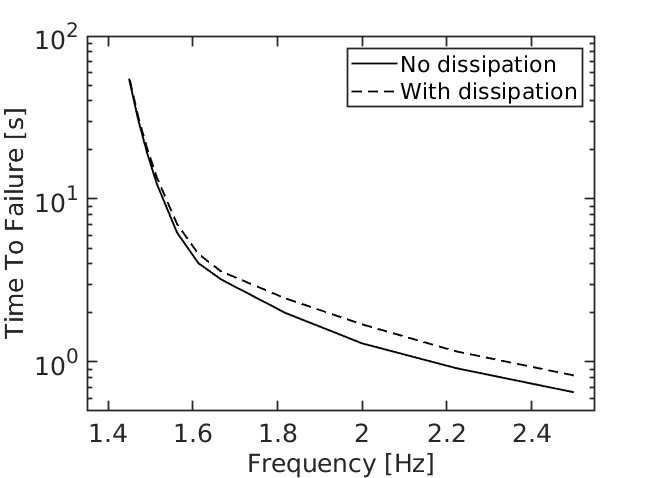
\includegraphics[width=0.8\columnwidth]{figures/TestCases/FrankaHand/time_to_failure_reference.png}
    \caption{Time to Failure $T_f$ with and without Hunt \& Crossley dissipation. Reference solutions
    with $\delta t = 0.2\text{ ms}$.}
    \label{fig:ranka_reference_solutions}
\end{figure}

We compute the relative error in $T_f$ against the reference solutions (Fig.
\ref{fig:franka_time_to_failure_errors}), with positive values indicating
overestimation. At $\delta t=0.2\text{ ms}$ and zero dissipation, Lagged and
Similar solutions differ by less than 0.5\% (Fig.
\ref{fig:franka_time_to_failure_errors}, left), indicating that Similar's
\emph{gliding} contribution $\mu\delta t\Vert\vf{v}_t\Vert$ is negligible.

At large $\delta t=10\text{ ms}$ errors increase up to 50\% due to how
incredibly sensitive $T_f$ is. The goal however is to understand the relative
importance of each error contribution rather than a precise determination of
$T_f$. Without dissipation, truncation errors dominate, causing both
approximations to underpredict $T_f$. $T_f$ with Similar is slightly larger
compared to Lagged (error is less negative), as the gliding effect introduces
transient penetrations $\delta t\mu\Vert\vf{v}_t\Vert$ that increase the mean
grasp force.

\begin{figure}[!h]
    \centering
    %trim={<left> <lower> <right> <upper>}
    \adjincludegraphics[height=0.38\columnwidth,trim={0 0 {0.05\width} 0},clip]{figures/TestCases/FrankaHand/error_in_time_to_failure_no_damping.png}
    \adjincludegraphics[height=0.38\columnwidth,trim={0 0 {0.05\width} 0},clip]{figures/TestCases/FrankaHand/error_in_time_to_failure_with_damping.png}
    \caption{\label{fig:franka_time_to_failure_errors} Relative error in $T_f$ without
    (left) and with (right) dissipation. Positive values indicates $T_f$ is over predicted.}
\end{figure}

From Fig. \ref{fig:franka_time_to_failure_errors} (left), Similar's gliding is
negligible at 0.2~ms. Thus, the 30\% error increase in Fig.
\ref{fig:franka_time_to_failure_errors} (right) is fully attributed to
compliance modulation, comparable to truncation error.

At $\delta t=10\text{ ms}$, Lagged's error remains nearly unchanged with or
without dissipation. Similar's error decreases due to the cancellation of two
effects: truncation errors causing $T_f$ underestimation (Fig.
\ref{fig:franka_time_to_failure_errors}, left) and compliance modulation leading
to overprediction (Fig. \ref{fig:franka_time_to_failure_errors}, right).

At large time steps for interactive simulation, both models exhibit similar
error magnitudes. Even in this highly dynamic case, Lagged's weak coupling
does not degrade grasp performance. Since Lagged eliminates \emph{gliding} and
\emph{compliance modulation}, we recommend it over Similar and SAP.
